\begin{figure}[ht]
	\centering
	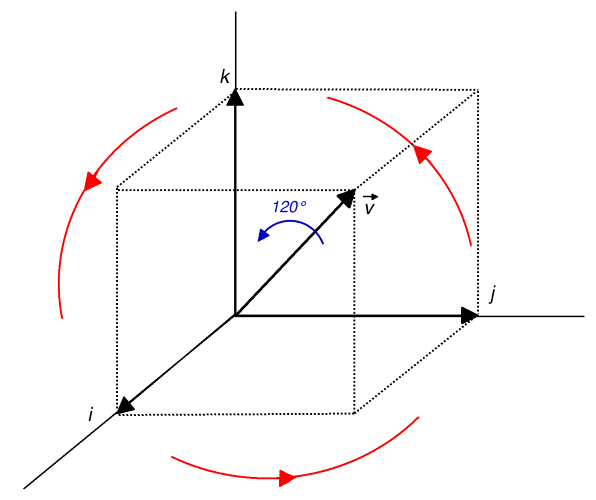
\includegraphics[height=5cm]{ressources/rotation_diagonale}\hfill
	\caption{Une rotation de \ang{120} autour de la première diagonale permute i, j et k circulairement.}
	\label{exemple}
\end{figure}

Considérons la rotation $f$ autour de l'axe dirigé par $ \vec{u} = i + j + k $ et 
d'angle \ang{120}, c'est-à-dire $\frac{2 \pi}{3}$ radians.

\[
\alpha = \frac{2 \pi}{3}
\]

La norme de $\vec{u}$ est $\sqrt{3}$, le demi-angle est $\frac{\pi}{3}$ (\ang{60}), le cosinus
de ce demi-angle est $\frac{1}{2}$, (cos \ang{60} = 0.5) et son sinus est $\sqrt{\frac{3}{2}}$,
(sin \ang{60} $\approx$ 0,866). Nous devons donc conjuguer avec le quaternion unitaire:

\begin{align*}
  q & = \cosad + \sinad \cdot \frac{1}{\lVert\vec{u}\rVert} \vec{u} \\
 & = \cos \frac{\pi}{3} + \sin \frac{\pi}{3} \cdot \frac{1}{\sqrt{3}} \vec{u} \\
 & = \frac{1}{2} + \frac{\sqrt{3}}{2} \cdot \frac{1}{\sqrt{3}} \vec{u} \\
 & = \frac{1}{2} + \frac{\sqrt{3}}{2} \cdot \frac{i + j + k}{\sqrt{3}} \\
 & = \frac{1 + i + j + k}{2}
\end{align*}

Si $f$ est la fonction de rotation,

\[
	f(ai+bj+ck) = q(ai+bj+ck)q^-1^-1
\]

On peut prouver que l'on obtient l'inverse d'un quaternion unitaire simplement en
changeant le signe de ses coordonnées imaginaires. En conséquence, 

\[
	q^-1 = \frac{1 - i - j - k}{2}
\]

et

\[
	f(ai+bj+ck) = \frac{1 - i - j - k}{2} (ai+bj+ck)\frac{1 - i - j - k}{2}
\]

En appliquant les règles ordinaires de calcul avec les quaternions, on obtient

\[
	f(ai+bj+ck) = ci + aj + ck
\]

Comme on s'y attendait, la rotation revient à tenir un cube par un de ses sommets, 
puis à le faire tourner de \ang{120} selon la diagonale la plus longue qui passe par ce point. On observe comment les trois axes subissent une \emph{permutation circulaire}.

\begin{dem}[title=Démonstration]{}{}
Prouvons le résultat précédent : 
En développant l'expression de $f$ (en deux étapes) et en appliquant les règles :

\[
	ij = k, ji = -k,
	jk=i, kj = -i,
	ki=k, ik=-j,
	i^2=j^2=k^2=-1
\]

on obtient:

\begin{align*}
	f(ai+bj+ck) &= \frac{1+i+j+k}{2}(ai+bj+ck)\frac{1-i-j-k}{2}
	(1 - i - j - k) \\
	&= \qter((ai+bj+ck)+(-a+bk-cj)+(-ak-b+ci)+(aj-bi-c)) \\
	(1 - i - j - k) \\
	&= \qter ((-a-b-c) + (a-b+c)i + (a+b-c)j + (-a+b+c)k) \\
	(1 - i - j - k)\\
	\text{...}
	&= ci + aj + bk
\end{align*}

Ce qui est bien le résultat annoncé. On voit que de tels calculs sont 
relativement fastidieux à faire à la main, mais dans un programme d'ordinateur, 
cela se résume à appeler deux fois la routine de multiplication de quaternions.

\end{dem}
